% Options for packages loaded elsewhere
\PassOptionsToPackage{unicode}{hyperref}
\PassOptionsToPackage{hyphens}{url}
%
\documentclass[
  english,
  man]{apa6}
\usepackage{lmodern}
\usepackage{amsmath}
\usepackage{ifxetex,ifluatex}
\ifnum 0\ifxetex 1\fi\ifluatex 1\fi=0 % if pdftex
  \usepackage[T1]{fontenc}
  \usepackage[utf8]{inputenc}
  \usepackage{textcomp} % provide euro and other symbols
  \usepackage{amssymb}
\else % if luatex or xetex
  \usepackage{unicode-math}
  \defaultfontfeatures{Scale=MatchLowercase}
  \defaultfontfeatures[\rmfamily]{Ligatures=TeX,Scale=1}
\fi
% Use upquote if available, for straight quotes in verbatim environments
\IfFileExists{upquote.sty}{\usepackage{upquote}}{}
\IfFileExists{microtype.sty}{% use microtype if available
  \usepackage[]{microtype}
  \UseMicrotypeSet[protrusion]{basicmath} % disable protrusion for tt fonts
}{}
\makeatletter
\@ifundefined{KOMAClassName}{% if non-KOMA class
  \IfFileExists{parskip.sty}{%
    \usepackage{parskip}
  }{% else
    \setlength{\parindent}{0pt}
    \setlength{\parskip}{6pt plus 2pt minus 1pt}}
}{% if KOMA class
  \KOMAoptions{parskip=half}}
\makeatother
\usepackage{xcolor}
\IfFileExists{xurl.sty}{\usepackage{xurl}}{} % add URL line breaks if available
\IfFileExists{bookmark.sty}{\usepackage{bookmark}}{\usepackage{hyperref}}
\hypersetup{
  pdftitle={Replication of Thinking of You: How second person pronouns shape cultural success},
  pdfauthor={Derek Maldonado1},
  pdflang={en-EN},
  pdfkeywords={language, pronouns, entertainment, success},
  hidelinks,
  pdfcreator={LaTeX via pandoc}}
\urlstyle{same} % disable monospaced font for URLs
\usepackage{graphicx}
\makeatletter
\def\maxwidth{\ifdim\Gin@nat@width>\linewidth\linewidth\else\Gin@nat@width\fi}
\def\maxheight{\ifdim\Gin@nat@height>\textheight\textheight\else\Gin@nat@height\fi}
\makeatother
% Scale images if necessary, so that they will not overflow the page
% margins by default, and it is still possible to overwrite the defaults
% using explicit options in \includegraphics[width, height, ...]{}
\setkeys{Gin}{width=\maxwidth,height=\maxheight,keepaspectratio}
% Set default figure placement to htbp
\makeatletter
\def\fps@figure{htbp}
\makeatother
\setlength{\emergencystretch}{3em} % prevent overfull lines
\providecommand{\tightlist}{%
  \setlength{\itemsep}{0pt}\setlength{\parskip}{0pt}}
\setcounter{secnumdepth}{-\maxdimen} % remove section numbering
% Make \paragraph and \subparagraph free-standing
\ifx\paragraph\undefined\else
  \let\oldparagraph\paragraph
  \renewcommand{\paragraph}[1]{\oldparagraph{#1}\mbox{}}
\fi
\ifx\subparagraph\undefined\else
  \let\oldsubparagraph\subparagraph
  \renewcommand{\subparagraph}[1]{\oldsubparagraph{#1}\mbox{}}
\fi
% Manuscript styling
\usepackage{upgreek}
\captionsetup{font=singlespacing,justification=justified}

% Table formatting
\usepackage{longtable}
\usepackage{lscape}
% \usepackage[counterclockwise]{rotating}   % Landscape page setup for large tables
\usepackage{multirow}		% Table styling
\usepackage{tabularx}		% Control Column width
\usepackage[flushleft]{threeparttable}	% Allows for three part tables with a specified notes section
\usepackage{threeparttablex}            % Lets threeparttable work with longtable

% Create new environments so endfloat can handle them
% \newenvironment{ltable}
%   {\begin{landscape}\begin{center}\begin{threeparttable}}
%   {\end{threeparttable}\end{center}\end{landscape}}
\newenvironment{lltable}{\begin{landscape}\begin{center}\begin{ThreePartTable}}{\end{ThreePartTable}\end{center}\end{landscape}}

% Enables adjusting longtable caption width to table width
% Solution found at http://golatex.de/longtable-mit-caption-so-breit-wie-die-tabelle-t15767.html
\makeatletter
\newcommand\LastLTentrywidth{1em}
\newlength\longtablewidth
\setlength{\longtablewidth}{1in}
\newcommand{\getlongtablewidth}{\begingroup \ifcsname LT@\roman{LT@tables}\endcsname \global\longtablewidth=0pt \renewcommand{\LT@entry}[2]{\global\advance\longtablewidth by ##2\relax\gdef\LastLTentrywidth{##2}}\@nameuse{LT@\roman{LT@tables}} \fi \endgroup}

% \setlength{\parindent}{0.5in}
% \setlength{\parskip}{0pt plus 0pt minus 0pt}

% \usepackage{etoolbox}
\makeatletter
\patchcmd{\HyOrg@maketitle}
  {\section{\normalfont\normalsize\abstractname}}
  {\section*{\normalfont\normalsize\abstractname}}
  {}{\typeout{Failed to patch abstract.}}
\patchcmd{\HyOrg@maketitle}
  {\section{\protect\normalfont{\@title}}}
  {\section*{\protect\normalfont{\@title}}}
  {}{\typeout{Failed to patch title.}}
\makeatother
\shorttitle{Replication of Thinking of YOU}
\keywords{language, pronouns, entertainment, success\newline\indent Word count: X}
\DeclareDelayedFloatFlavor{ThreePartTable}{table}
\DeclareDelayedFloatFlavor{lltable}{table}
\DeclareDelayedFloatFlavor*{longtable}{table}
\makeatletter
\renewcommand{\efloat@iwrite}[1]{\immediate\expandafter\protected@write\csname efloat@post#1\endcsname{}}
\makeatother
\usepackage{lineno}

\linenumbers
\usepackage{csquotes}
\ifxetex
  % Load polyglossia as late as possible: uses bidi with RTL langages (e.g. Hebrew, Arabic)
  \usepackage{polyglossia}
  \setmainlanguage[]{english}
\else
  \usepackage[shorthands=off,main=english]{babel}
\fi
\ifluatex
  \usepackage{selnolig}  % disable illegal ligatures
\fi
\newlength{\cslhangindent}
\setlength{\cslhangindent}{1.5em}
\newlength{\csllabelwidth}
\setlength{\csllabelwidth}{3em}
\newenvironment{CSLReferences}[3] % #1 hanging-ident, #2 entry spacing
 {% don't indent paragraphs
  \setlength{\parindent}{0pt}
  % turn on hanging indent if param 1 is 1
  \ifodd #1 \everypar{\setlength{\hangindent}{\cslhangindent}}\ignorespaces\fi
  % set entry spacing
  \ifnum #2 > 0
  \setlength{\parskip}{#2\baselineskip}
  \fi
 }%
 {}
\usepackage{calc}
\newcommand{\CSLBlock}[1]{#1\hfill\break}
\newcommand{\CSLLeftMargin}[1]{\parbox[t]{\csllabelwidth}{#1}}
\newcommand{\CSLRightInline}[1]{\parbox[t]{\linewidth - \csllabelwidth}{#1}}
\newcommand{\CSLIndent}[1]{\hspace{\cslhangindent}#1}

\title{Replication of Thinking of You: How second person pronouns shape cultural success}
\author{Derek Maldonado\textsuperscript{1}}
\date{}


\authornote{

Derek Maldonado, Graduate student, experimental psychology, Brooklyn College of the City University of New York.

The authors made the following contributions. Derek Maldonado: Conceptualization, Writing - Original Draft Preparation, Writing - Review \& Editing.

Correspondence concerning this article should be addressed to Derek Maldonado, 2900 Bedford Ave, Brooklyn, 11210. E-mail: \href{mailto:derekmaldonado24@gmail.com}{\nolinkurl{derekmaldonado24@gmail.com}}

}

\affiliation{\vspace{0.5cm}\textsuperscript{1} Brooklyn College}

\abstract{
How are you affected by the music you listen to? This experiment attempts to replicate the work done by Packard and Berger (2020) in study two where they examined the use of the word ``you'' in popular music. The hypothesis was that there would be a significant increase in the score a person gave a song that featured the word ``you'' and seemed to point to the listener more than songs from other points of view. The data showed this hypothesis to be somewhat correct in the sense the word did lead to an increase in musical enjoyment.
}



\begin{document}
\maketitle

Why do people enjoy some songs more than others? How is it that a specific piece of music can break through the zeitgeist and become a number one hit. An experiment done by Packard and Berger (2020) attempts to examine this phenomenon by finding a connecting piece between all the most popular music floating in people's minds.The word ``you'' carries a specific connotation, as it can make the audience member feel part of the song being listened to and increase their enjoyment. In their second of four studies, they directly asked participants about songs sitting in their head and how much they enjoy or dislike them.

\hypertarget{methods}{%
\section{Methods}\label{methods}}

We report how we determined our sample size, all data exclusions (if any), all manipulations, and all measures in the study.

\hypertarget{participants}{%
\subsection{Participants}\label{participants}}

There were 188 participants found through Amazon's Mechanical Turk platform.

\hypertarget{material}{%
\subsection{Material}\label{material}}

The study was completed through a online survey.

\hypertarget{procedure}{%
\subsection{Procedure}\label{procedure}}

The participants were asked to name a song they heard recently and write down the song as well as the artist that performed the song. They were then asked to rate the song based on two questions: how much they liked the song as well as how much they enjoyed listening to the song. These two answers were then aggregated into a data set.
They then averaged the scores of the two questions and compared those scores to the number of times the word you was used in the song.

\hypertarget{data-analysis}{%
\subsection{Data analysis}\label{data-analysis}}

We used R (Version 4.0.2; R Core Team, 2020) and the R-package \emph{papaja} (Version 0.1.0.9997; Aust \& Barth, 2020) for all our analyses.

\begin{verbatim}
## Warning: package 'gt' was built under R version 4.0.3
\end{verbatim}

\begin{verbatim}
## Warning: package 'tibble' was built under R version 4.0.3
\end{verbatim}

\begin{verbatim}
## Warning: package 'readr' was built under R version 4.0.3
\end{verbatim}

\begin{verbatim}
## Warning: package 'glue' was built under R version 4.0.3
\end{verbatim}

\begin{verbatim}
## 
##  Pearson's product-moment correlation
## 
## data:  rating and yoused
## t = 2.4776, df = 186, p-value = 0.01412
## alternative hypothesis: true correlation is not equal to 0
## 95 percent confidence interval:
##  0.03656476 0.31382252
## sample estimates:
##       cor 
## 0.1787397
\end{verbatim}

\begin{verbatim}
## [1] 0.03194788
\end{verbatim}

\hypertarget{results}{%
\section{Results}\label{results}}

The use of the word you and the participant's enjoyment of the song were found to be significantly positively correlated, r(186)=0.1787 p-value=0.01412.

\hypertarget{discussion}{%
\section{Discussion}\label{discussion}}

We successfully replicated study two and showed there to be statistically significant results. This shows there to be some possible correlation between the use of you and a person's enjoyment of a song. The big limitation of this second part of the study is that it is based only on songs a person is currently thinking of, meaning it is most likely focused on very popular songs already. The other aspects of the study do cover the other areas of musical understanding, create a full picture. It can be found in the references below.

\hypertarget{power-analysis}{%
\section{Power Analysis}\label{power-analysis}}

\begin{verbatim}
## Warning: package 'pwr' was built under R version 4.0.3
\end{verbatim}

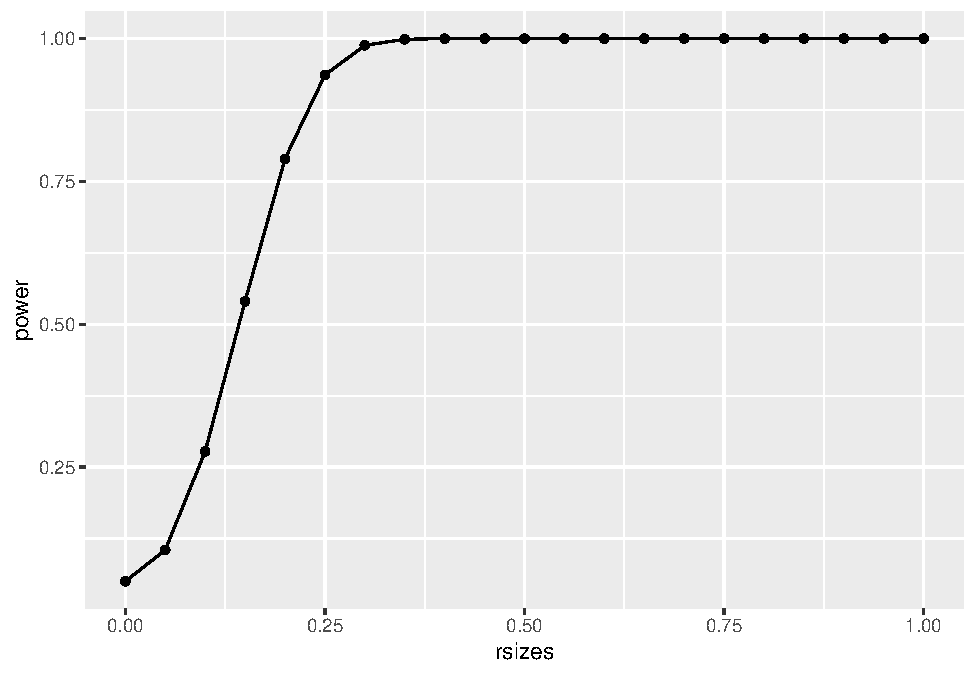
\includegraphics{finalprojectapa_files/figure-latex/unnamed-chunk-2-1.pdf}

We completed a power analysis with a n=188 and examining r values between 0 and 1 at steps of 0.05 to give us a clear curve. The analysis shows that with a large n, this experiment inherently has a high amount of power. As seen, at a r-value = 0.17 the expected power is around 0.75. With this, the experimenter can understandably reject the null with a p-value of 0.014, much lower than the 0.05 significance level in the power analysis.

This experiment can reach a higher level of power only by increasing the n.~With it being a correlational study, an increase in n should increase the power on principle as well as increase the acquired r-value if there is in fact a correlation as proposed.

\newpage

\hypertarget{references}{%
\section{References}\label{references}}

\begingroup
\setlength{\parindent}{-0.5in}
\setlength{\leftskip}{0.5in}

\hypertarget{refs}{}
\begin{CSLReferences}{1}{0}
\leavevmode\hypertarget{ref-R-papaja}{}%
Aust, F., \& Barth, M. (2020). \emph{{papaja}: {Create} {APA} manuscripts with {R Markdown}}. Retrieved from \url{https://github.com/crsh/papaja}

\leavevmode\hypertarget{ref-PackardBergerYou}{}%
Packard, G., \& Berger, J. (2020). Thinking of you: How second-person pronouns shape cultural success. \emph{Psychological Science}, \emph{31}(4), 397--407.

\leavevmode\hypertarget{ref-R-base}{}%
R Core Team. (2020). \emph{R: A language and environment for statistical computing}. Vienna, Austria: R Foundation for Statistical Computing. Retrieved from \url{https://www.R-project.org/}

\end{CSLReferences}

\endgroup


\end{document}
